\section{Generación de instancias del problema e instancias de entrenamiento} \label{chapter-implementacion:data}

\paragraph{} Dado el problema HCSP, surgen dos posibles maneras de utilizar una instancia del problema (dado por una matriz ETC) y su resolución (una planificación) en el contexto de aprendizaje automático. Una opción implica utilizar a la matriz ETC completa como entrada del clasificador de elección y, hacer que la salida esperada sea la planificación, es decir todas las asignaciones tarea-máquina esperadas. Esto constituye un problema de clasificación multiclase, y la desventaja principal que presenta es la de no permitir escalar en términos de máquinas o tareas. Esto implica que si un clasificador es entrenado para aprender a resolver el problema HCSP con instancias del problema de dimensión $M \times N$, no será aplicable para ninguna otra dimensión. La otra opción que se presenta, y la que fue escogida finalmente en este trabajo tomando como referencia el trabajo de \citet{savant-original}, es la de descomponer a una matriz ETC en varios ejemplos de entrenamiento. Por lo tanto, dado un ejemplo de entrenamiento bajo este paradigma, se tiene a la información asociada únicamente a una tarea como la entrada, y a la asignación tarea-máquina de esa tarea como la salida esperada. Esto causa que una instancia del problema (con su planificación asociada) de dimensión $M \times N$ se convierta en $M$ potenciales ejemplos de entrenamiento, y proporciona la posibilidad de escalar en términos de la cantidad de tareas a ejecutar. Esta oportunidad surge dado el hecho de que ahora un ejemplo de entrenamiento está limitado únicamente por la cantidad de máquinas, y se presenta con más detalle en la sección \ref{chapter-implementacion:clasificadores}.
% matriz entera
% matriz parcial


\paragraph{} Con el objetivo de generar ejemplos de entrenamiento y validación como los discutidos anteriormente para entrenar y evaluar a los clasificadores construidos, fue necesario desarrollar un componente de software que pudiera hacerlo a demanda. Este componente está conformado fundamentalmente por scripts, y en la Figura \ref{fig:diagrama-datos} se puede ver un diagrama de secuencia donde se explicita su funcionamiento. 

\paragraph{} Inicialmente, se utiliza un script extraído de \citet{bib-doctorado-nesmachnow} para generar instancias del problema, y se genera una solución para dicha instancia utilizando una implementación de Min-Min. % TODO tal vez agregar implementación en apéndice.
Estos elementos son persistidos directamente al sistema de archivos de manera iterativa, de acuerdo a la cantidad de ejemplos de entrenamiento que se deseen generar.
Una vez finalizada esta etapa, es necesario modificar la estructura de los datos generados, de manera de obtener aquella estructura soportada por los clasificadores de aprendizaje automático. Por lo tanto, se procede a tomar cada par constituido por una instancia del problema y su planificación esperada, y se generan tantos ejemplos de entrenamiento como tareas existan en la instancia del problema. Es decir que para una instancia del problema de dimensión $M \times N$ tendremos $M$ ejemplos de entrenamiento. Finalmente, se agrupan estos ejemplos de entrenamiento y se persisten en formato CSV para su uso posterior. Este formato es utilizado por ser el estándar soportado más comúnmente por las librerías de manejo de datos utilizadas.

\textsc{\begin{figure}[ht!]
	\centering
    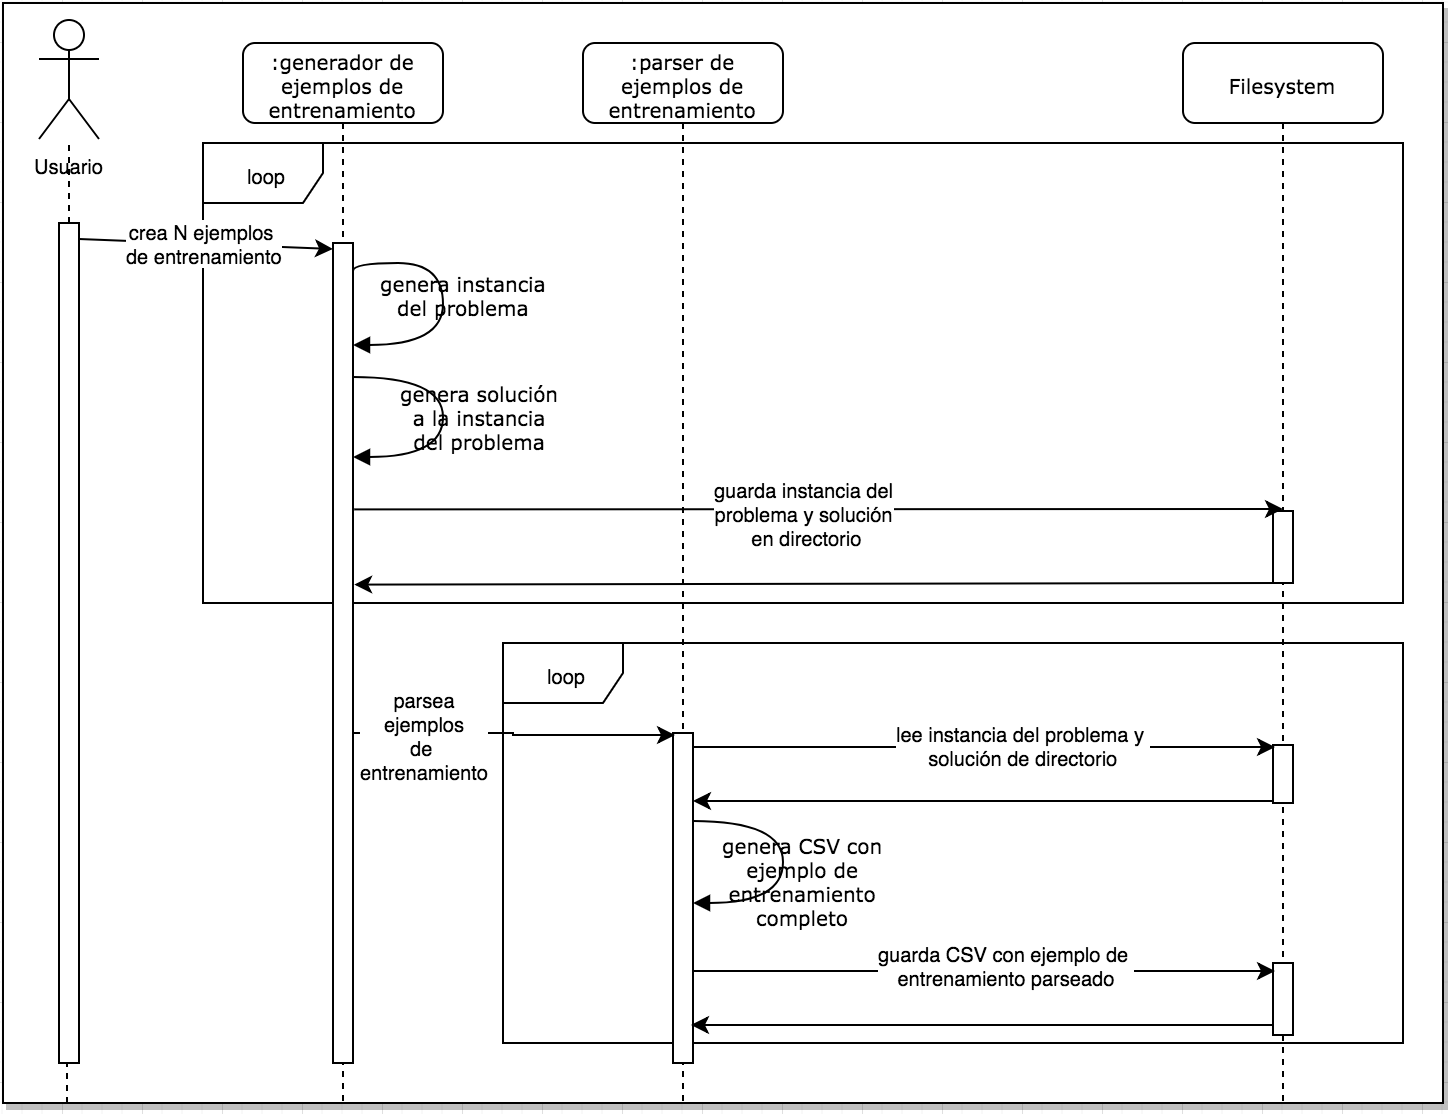
\includegraphics[width=.9\linewidth]{imagenes/implementacion/diagrama-datos.png}
	\caption{Diagrama de secuencia de generación de ejemplos de entrenamiento.}
	\label{fig:diagrama-datos}
\end{figure}}

\paragraph{} Este componente de software, como el resto de los aquí mencionados, fue desarrollado de manera de permitir su ejecución automatizada, a pesar de existir un usuario presente en el diagrama de secuencia. Dicho usuario puede bien ser un usuario final o un script encargado de invocar a este sistema. La posibilidad de automatización favorece la generación de ejemplos de entrenamiento a gran escala y de manera paralela mediante el uso de hilos. Además, se ofrece al usuario la posibilidad de determinar cuántas instancias del problema (con sus correspondientes soluciones) serán generadas, dónde se persisten, y las características de los tipos de instancias del problema a generar, como por ejemplo la dimensión de las mismas.